%
%===============>>  ГРУППА 8-1 МОДУЛЬ 8  <<=============
%
\setmodule{9}

%BEGIN_FOLD % ====>>_____ Занятие 1 _____<<====
\begin{class}[number=1]
	\begin{listofex}
		\item 
		\begin{minipage}[t]{\bodywidth}
			На рисунке \( AB = 4 \), \( BE = 8 \), \( DE = 5 \), прямая \( AB \) перпендикулярна прямой \( BD \), \( CD \) перпендикулярна \( BD \) и \( EA \) перпендикулярна \( EC \).	Найдите \( CD \). 
		\end{minipage}
		\hspace{0.02\linewidth}
		\begin{minipage}[t]{\picwidth}
			% TODO: \usepackage{graphicx} required
			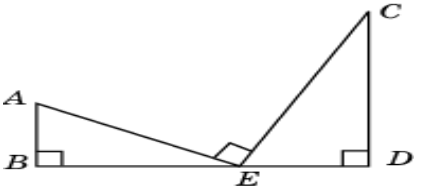
\includegraphics[align=t, width=\linewidth]{../../../../exercises/lists/pics/G81M9L1-1}
		\end{minipage}
		\item 
		\begin{minipage}[t]{\bodywidth}
			На рисунке \( DE = 10 \), \( CE = 8 \), \( BC = 12 \), угол \( BAC \) равен углу \(  EDC \). Найдите \( AB \).
		\end{minipage}
		\hspace{0.02\linewidth}
		\begin{minipage}[t]{\picwidth}
			% TODO: \usepackage{graphicx} required
			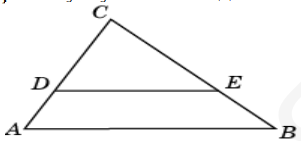
\includegraphics[align=t, width=\linewidth]{../../../../exercises/lists/pics/G81M9L1-2}
		\end{minipage}
		\item Через точки \( M \) и \( N \), принадлежащие сторонам \( AB \) и \( BC  \) треугольника \(  ABC \) соответственно, проведена прямая \( MN \), параллельная стороне \( AC \). Найдите длину \( CN \), если \( BC = 6 \), \( MN = 4 \) и \( AC = 9 \).
		\item  Прямая, параллельная основанию треугольника, делит его на треугольник и трапецию, площади которых относятся как 4:5. Периметр образовавшегося треугольника равен 20 см. Найдите периметр данного треугольника.
		\item Через вершину прямого угла прямоугольного треугольника с катетами 6 и 8 см проведен перпендикуляр к гипотенузе. Вычислите площади образовавшихся треугольников.		
		\item  В прямоугольном треугольнике \( ABC \) проведена высота \( CH \) к гипотенузе. \( CH=4 \), \( BH=3 \). Найдите катет \( AC \).		
		\item  Основание треугольника 15 см, а боковые стороны 13 и 14 см. Высота разделена в отношении 2:3 (считая от вершины) и через точку деления проведена прямая, параллельная основанию. Найдите площадь образовавшейся при этом трапеции. 
		\item Подобны ли треугольники \( ABC \) и \( A_1B_1C_1 \), если известно, что:
		
		\begin{tasks}(1)
			\task \( AB = 10 \) см; \( BC = 5 \) см; \( AC = 7 \) см; \( A_1B_1 = 15 \) см; \( B_1C_1 = 7,5 \) см; \( A_1C_1 = 9,5 \) см?
			\task \( \angle A = 37\degree \), \( \angle B = 48\degree \), \( \angle C_1 = 95\degree \), \( \angle B_1 = 48\degree \)?
			\task 	\( AB = 10  \) см, \( BC = 8 \) см, \( A_1B_1 = 5 \) см, \( A_1C_1 = 3 \) см, \( \angle C = \angle C_1 = 90\degree \)?
		\end{tasks}
		\item В прямоугольном треугольнике проведена высота к гипотенузе. Гипотенуза треугольника делится этой высотой на отрезки длиной 9 и 289. Найдите эту высоту и катеты треугольника.
		\item В прямоугольном треугольнике катет равен 4, а проекция этого катета на гипотенузу равна 2. Найдите гипотенузу, второй катет и его проекцию на гипотенузу.
		\item \( M \) и \( K \) соответственно середины сторон \( AB \) и \( BC \) треугольника \( ABC \). Найдите \( MK \), если \( AC = 7 \) см.
		\item В треугольнике \( ABC \) \( О \) и \( P \) --- середины сторон \( BC \) и \( AC \) соответственно. Длина отрезка \( OP \) равна 2,7 см. Найдите \( AB \).
		
	
	\end{listofex}
\end{class}
%END_FOLD

%BEGIN_FOLD % ====>>_____ Занятие 2 _____<<====
\begin{class}[number=2]
	\begin{listofex}
		\item 
		\begin{minipage}[t]{\bodywidth}
			В прямоугольном треугольнике биссектриса острого угла делит катет на отрезки \( 10 \) см и \( 6 \) см. Найдите периметр треугольника.
		\end{minipage}
		\hspace{0.02\linewidth}
		\begin{minipage}[t]{\picwidth}
			% TODO: \usepackage{graphicx} required
			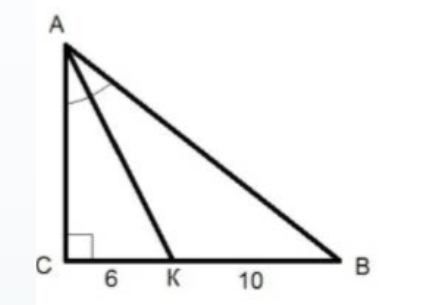
\includegraphics[align=t, width=\linewidth]{../../../../exercises/lists/pics/G81M9L2-1}
		\end{minipage}
	\item 
	\begin{minipage}[t]{\bodywidth}
		Определить длину \( AD\) геометрической фигуры на рисунке.
	\end{minipage}
	\hspace{0.02\linewidth}
	\begin{minipage}[t]{\picwidth}
		% TODO: \usepackage{graphicx} required
		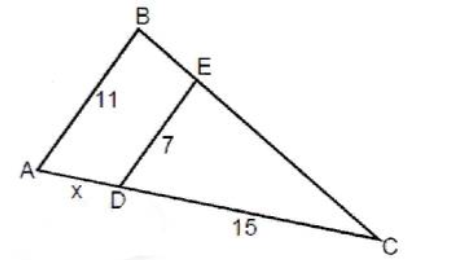
\includegraphics[align=t, width=\linewidth]{../../../../exercises/lists/pics/G81M9L2-2}
	\end{minipage}
	\item В прямоугольном треугольнике \( ABC \) высота, проведенная к гипотенузе \( AB \), делит ее на части, разность длин которых равна \( 6 \) см, а высота \( CH \) равна \( 4 \). Вычислите длину гипотенузы.
	\item В равнобедренном треугольнике \( ABC \) высота \( AE \), опущенная на боковую сторону, делит ее на отрезки \( 7 \) см и \( 2 \) см, считая от вершины. Вычислите основания треугольника.
	\item Биссектриса \( AD \) угла треугольника \( ABC \) делит противоположную сторону на отрезки \( 7 \) см и \( 5 \) см. Периметр треугольника равен \( 36 \) см. Вычислите стороны треугольника.
	\item В треугольнике АВС высота \( CH \) и медиана \( CM \) делят угол \( C \) на три равные части. Докажите, что угол \( C \) – прямой.
	\item Точка \( E \) лежит на стороне \( AC \) треугольника \( ABC \), причём \( \dfrac{EC}{AE} = 2 \). Точка \( D \) лежит на \( BC \), причём \( ED\parallel AB \). Найдите \( AB \), если \( ED = \dfrac{4}{3} \).
	\item 
	\begin{minipage}[t]{\bodywidth}
		 Дан прямоугольный треугольник  \( \Delta ABC\)  \( \angle C = 90\degree  \), \( CH \) – высота. \( AH=9 \), \( BH = 16 \). Найти \( BC \), \( AC \), \( CH \).
	\end{minipage}
	\hspace{0.02\linewidth}
	\begin{minipage}[t]{\picwidth}
		% TODO: \usepackage{graphicx} required
		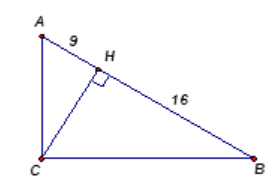
\includegraphics[align=t, width=\linewidth]{../../../../exercises/lists/pics/G81M9L2-3}
	\end{minipage}
	\item Найдите периметр прямоугольного треугольника, высота которого делит гипотенузу на отрезки длиной \( 4,5 \) см и \( 8 \) см.
	\item В треугольнике, стороны которого равны \( 15 \), \( 20 \), \( 25 \), проведена высота к его большей стороне. Найдите отрезки, на которые высота делит эту сторону.
	\end{listofex}
\end{class}
%END_FOLD

%BEGIN_FOLD % ====>>_ Домашняя работа 1 _<<====
\begin{homework}[number=1]
	\begin{listofex}
		\item 
		\begin{minipage}[t]{\bodywidth}
			Дано: \( \angle A = \angle B \), \( CO = 4 \), \( DO = 6 \), \( AO = 5  \). Найти:\begin{tasks}(2)
			\task \( OB \)
			\task \( AC : BD \) 
			\task \( S_{AOC} : S_{BOD} \)
		\end{tasks}
		\end{minipage}
		\hspace{0.02\linewidth}
		\begin{minipage}[t]{\picwidth}
			% TODO: \usepackage{graphicx} required
			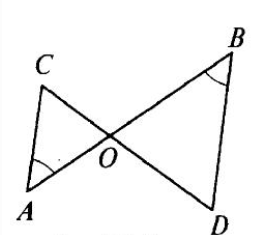
\includegraphics[align=t, width=\linewidth]{../../../../exercises/lists/pics/G81M9H1-1}
		\end{minipage}
		\item На сторонах \( AB \) и \( BC \) треугольника \( ABC \) отмечены точки \( K \) и \( E \) так, что \( AK=KB \), \( BE=CE \), \( KE=6 \) см. Найдите сторону \( AC \).
		\item  Прямая, параллельная основанию треугольника, делит его на треугольник и трапецию, площади которых относятся как \( 4:5 \). Периметр образовавшегося треугольника равен \( 20 \) см. Найдите периметр.
		\item Человек ростом \( 1,7 \) м стоит на расстоянии \( 8 \) метров от столба, на котором висит фонарь. Тень человека равна \( 4 \) метрам. На какой высоте в метрах расположен фонарь?
		\item Отрезки \( KE \) и \( MN \) пересекаются в точке \( O \), так что отрезок \( KM \) параллелен отрезку \( NE \). Докажите, что треугольники \( KMO \) и \( NEO \) подобны. Найдите \( KM \), если \( ON=6 \) см, \( MO=12 \) см, \( NE=18 \) см.
	\end{listofex}
\end{homework}
%END_FOLD

%BEGIN_FOLD % ====>>_____ Занятие 3 _____<<====
\begin{class}[number=3]
	\begin{listofex} 
		\item 
		\begin{minipage}[t]{\bodywidth}
			На рисунке \( KP = 6 \), \( LP = 4 \), \( NP = 8 \), \( MN \)
		параллельна \(  KL \). Найдите \( MP \). 
		\end{minipage}
		\hspace{0.02\linewidth}
		\begin{minipage}[t]{\picwidth}
			% TODO: \usepackage{graphicx} required
			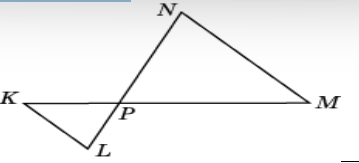
\includegraphics[align=t, width=1.3\linewidth]{../../../../exercises/lists/pics/G81M9L3-1}
		\end{minipage}
		\item 
		\begin{minipage}[t]{\bodywidth}
			 Человек ростом \( 1,8 \) м стоит на расстоянии \( 12 \) м от столба, на котором висит фонарь на высоте \(  5,4 \)
		м. Найдите длину тени человека в метрах.
		\end{minipage}
		\hspace{0.02\linewidth}
		\begin{minipage}[t]{\picwidth}
			% TODO: \usepackage{graphicx} required
			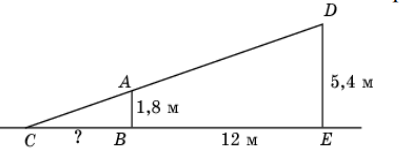
\includegraphics[align=t, width=1.6\linewidth]{../../../../exercises/lists/pics/G81M9L3-2}
		\end{minipage}
		\item 
		\begin{minipage}[t]{\bodywidth}
			Используя данные, приведенные на рисунке,
			найдите высоту мачты \( AB \). 
		\end{minipage}
		\hspace{0.02\linewidth}
		\begin{minipage}[t]{\picwidth}
			% TODO: \usepackage{graphicx} required
			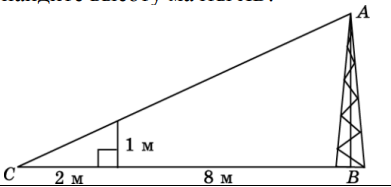
\includegraphics[align=t, width=1.5\linewidth]{../../../../exercises/lists/pics/G81M9L3-3}
		\end{minipage}
		\item 
		\begin{minipage}[t]{\bodywidth}
			Используя данные, приведенные на рисунке,
			найдите ширину \( AB \) реки.
		\end{minipage}
		\hspace{0.02\linewidth}
		\begin{minipage}[t]{\picwidth}
			% TODO: \usepackage{graphicx} required
			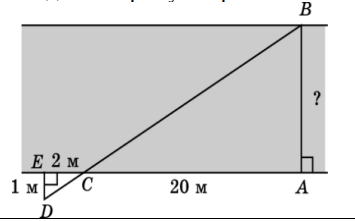
\includegraphics[align=t, width=1.5\linewidth]{../../../../exercises/lists/pics/G81M9L3-4}
		\end{minipage}
		\item 
		\begin{minipage}[t]{\bodywidth}
			Используя данные, приведенные на рисунке,
			найдите расстояние \( AB \) от лодки \( A \) до берега \( b \).
		\end{minipage}
		\hspace{0.02\linewidth}
		\begin{minipage}[t]{\picwidth}
			% TODO: \usepackage{graphicx} required
			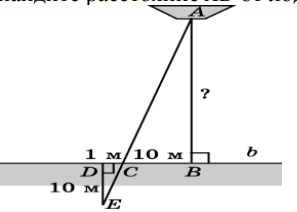
\includegraphics[align=t, width=1.5\linewidth]{../../../../exercises/lists/pics/G81M9L3-5}
		\end{minipage}
		\item Углы \( A \)   и \( B \)   треугольника \( ABC \)   равны углам \( A_1 \)   и \(  B_1 \)   треугольника \( A_1B_1C_1 \)   соответственно. Известно, что \( AB = 4 \),   \( AC = 8 \),  \(  A_1C_1 = 4 \)   и \( B_1C_1 =3 \).   Найдите сумму периметров треугольников \(  ABC \)   и \( A_1B_1C_1 \).  
		\item Сторона \( AB \) треугольника \( ABC \) разделена на три равные части через точки деления проведены прямые, параллельные стороне \( BC \). Найдите отрезки этих прямых, заключенные внутри треугольника, если \( BC=12 \).
		\item На стороне \( AC \) треугольника \( ABC \) отложен отрезок \( AM \), равный третьей части стороны \( AB \), а на стороне \( AB \) --- отрезок \( AN \), равный третьей части стороны \( AC \). Найдите \( MN \), если \( BC=15 \).
		\item   Через точку \( L \) на стороне \( BC \) треугольника \( ABC \) проведены прямые, параллельные сторонам \( AB \) и \( AC \) и пересекающие эти стороны соответственно в точках \( K \) и \( M \). Известно, что \( BL:LC=1:3 \), \( AB=12 \) и \( AC=18 \). Найдите стороны четырехугольника \( AKLM \).
	\end{listofex}
\end{class}
%END_FOLD

%BEGIN_FOLD % ====>>_____ Занятие 4 _____<<====
\begin{class}[number=4]
	\begin{listofex}
		\item Точка \( H \) является основанием высоты, проведённой из вершины прямого угла \( B \) треугольника \( ABC \) к гипотенузе \( AC \). Найдите \( AB \), если \( AH = 5 \), \( AC = 20 \).
		\item  Отрезки \( AB \) и \( DC \) лежат на параллельных прямых, а отрезки \( AC \) и \( BD \) пересекаются в точке \( M \). Найдите \( MC \), если \( AB = 10 \), \( DC = 25 \), \( AC = 56  \).
		\item Прямая, параллельная стороне \( AC \) треугольника \( ABC \), пересекает стороны \( AB \) и \( BC \) в точках \( M \) и \( N \) соответственно. Найдите \( BN \), если \( MN = 13 \), \( AC = 65 \), \( NC = 28 \).
		\item Высота треугольника разбивает его основание на два отрезка с длинами \( 8 \) и \( 9 \). Найдите длину этой высоты, если известно, что другая высота треугольника делит ее пополам.
		\item Боковая сторона треугольника разделена на пять равных частей, через точки деления проведены прямые, параллельные основанию.
		Найдите отрезки этих прямых, заключённые между боковыми сторонами, если основание равно \( 20 \).
		\item В треугольнике \( ABC \) проведена прямая \( BD \) так, что  \(  \angle ABD = \angle ACB \).  Найдите отрезки \( AD \) и \( DC \), если  \( AB = 2   \) и  \( AC = 4 \).
		\item Докажите, что высота прямоугольного треугольника, проведённая из вершины прямого угла, разбивает треугольник на два подобных треугольника.
		\item Точки \( M \) и \( K \) лежат на сторонах соответственно \( AB \) и \( BC \) треугольника \( ABC \), отрезки \( AK \) и \( CM \) пересекаются в точке \( P \). Известно, что каждый из отрезков \( AK \) и \( CM \) делится точкой \( P \) в отношении  \( 2 : 1 \),  считая от вершины. Докажите, что \( AK \) и \( CM \) – медианы треугольника.
		\item На стороны \( BC \) и \( CD \) параллелограмма \( ABCD \) (или на их продолжения) опущены перпендикуляры \( AM \) и \( AN \).
		Докажите, что треугольник \( MAN \) подобен треугольнику \( ABC \).
		\item Внутри прямого угла дана точка \( M \), расстояния которой от сторон угла равны \( 4 \) и \( 8 \). Прямая, проходящая через точку \( M \), отсекает от прямого угла треугольник с площадью \( 100 \). Найдите катеты треугольника.
	\end{listofex}
\end{class}
%END_FOLD

%BEGIN_FOLD % ====>>_ Домашняя работа 2 _<<====
\begin{homework}[number=2]
	\begin{listofex}
		\item  Большая сторона треугольника равна \( 18 \). Найдите остальные стороны треугольника, если стороны подобного ему треугольника равны \( 4 \), \( 6 \), \( 9 \).
		\item Найдите стороны треугольника \( ABC \), если он подобен трегольнику \( A_1B_1C_1 \) со сторонами \( 8 \), \( 16 \),\( 18 \) и \( S_{ABC}:S_{A_1B_1C_1}=1:4 \).
		\item Стороны треугольника равны \( 5 \), \( 6 \), \( 7 \). Найдите стороны другого треугольника, подобного данному, если периметр его равен \( 54 \).
		\item В остроугольном треугольнике \( ABC \) проведены высоты \( AA_1 \) и \( BB_1 \). Докажите, что  \( A_1C\cdot BC = B_1C\cdot AC \).
	\end{listofex}
\end{homework}
%END_FOLD

%BEGIN_FOLD % ====>>_____ Занятие 5 _____<<====
\begin{class}[number=5]
	\begin{listofex}
		\item 
		\begin{minipage}[t]{\bodywidth}
			Треугольники \( ABC \) и \( A_1B_1C_1 \) подобны. Найдите сторону \( AC \).
		\end{minipage}
		\hspace{0.02\linewidth}
		\begin{minipage}[t]{\picwidth}
			% TODO: \usepackage{graphicx} required
			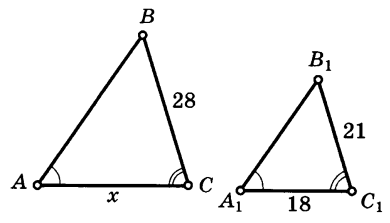
\includegraphics[align=t, width=1.5\linewidth]{../../../../exercises/lists/pics/G81M9L5-2}
		\end{minipage}
		\item 
		\begin{minipage}[t]{\bodywidth}
			Треугольники \( QMR \) и \( Q_1M_1R_1 \) подобны. Периметр треугольника \(  M_1Q_1R_1 \) равен \( 100 \).
		\end{minipage}
		\hspace{0.02\linewidth}
		\begin{minipage}[t]{\picwidth}
			% TODO: \usepackage{graphicx} required
			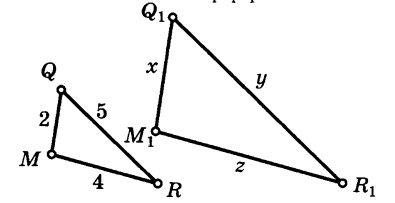
\includegraphics[align=t, width=1.5\linewidth]{../../../../exercises/lists/pics/G81M9L5-3}
		\end{minipage}
		\item 
		\begin{minipage}[t]{\bodywidth}
			Треугольники, изображенные на рисунке, подобны. Найдите стороны большего треугольника, если известно, что \( KL:LM:KM=6:7:5 \).
		\end{minipage}
		\hspace{0.02\linewidth}
		\begin{minipage}[t]{\picwidth}
			% TODO: \usepackage{graphicx} required
			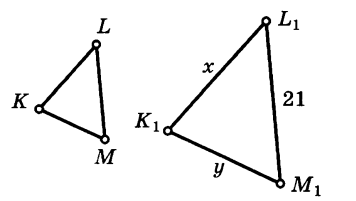
\includegraphics[align=t, width=1.5\linewidth]{../../../../exercises/lists/pics/G81M9L5-4}
		\end{minipage}
		\item
		\begin{minipage}[t]{\bodywidth}
			Найдите \( x \), \( y \).
		\end{minipage}
		\hspace{0.02\linewidth}
		\begin{minipage}[t]{\picwidth}
			% TODO: \usepackage{graphicx} required
			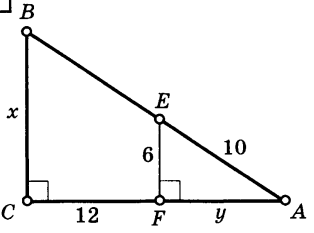
\includegraphics[align=t, width=\linewidth]{../../../../exercises/lists/pics/G81M9L5-5}
		\end{minipage}
		\item
		\begin{minipage}[t]{\bodywidth}
			Найдите \( x \), \( y \).
		\end{minipage}
		\hspace{0.02\linewidth}
		\begin{minipage}[t]{\picwidth}
			% TODO: \usepackage{graphicx} required
			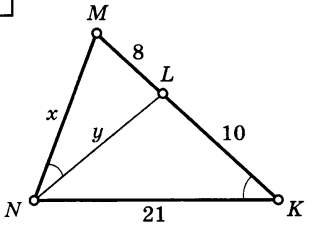
\includegraphics[align=t, width=\linewidth]{../../../../exercises/lists/pics/G81M9L5-6}
		\end{minipage}
		\item
		\begin{minipage}[t]{\bodywidth}
			Найдите \( x \), \( y \).
		\end{minipage}
		\hspace{0.02\linewidth}
		\begin{minipage}[t]{\picwidth}
			% TODO: \usepackage{graphicx} required
			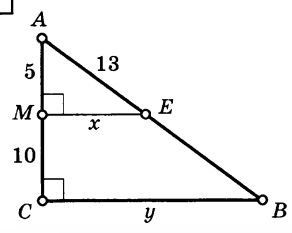
\includegraphics[align=t, width=\linewidth]{../../../../exercises/lists/pics/G81M9L5-7}
		\end{minipage}
		\item
		\begin{minipage}[t]{\bodywidth}
			Найдите \( x \), \( y \). Известно, что \( ON=12 \).
		\end{minipage}
		\hspace{0.02\linewidth}
		\begin{minipage}[t]{\picwidth}
			% TODO: \usepackage{graphicx} required
			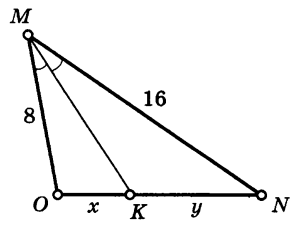
\includegraphics[align=t, width=\linewidth]{../../../../exercises/lists/pics/G81M9L5-8}
		\end{minipage}
		\item 
		\begin{minipage}[t]{\bodywidth}
			Укажите пары подобных треугольников и докажите их подобие.
		\end{minipage}
		\hspace{0.02\linewidth}
		\begin{minipage}[t]{\picwidth}
			% TODO: \usepackage{graphicx} required
			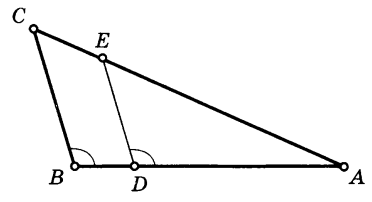
\includegraphics[align=t, width=\linewidth]{../../../../exercises/lists/pics/G81M9L5-9}
		\end{minipage}
		\item 
		\begin{minipage}[t]{\bodywidth}
			Треугольник \( KMN \) прямоугольный, \( KF \) его высота. Найдите пару подобных треугольников и докажите их подобие.
		\end{minipage}
		\hspace{0.02\linewidth}
		\begin{minipage}[t]{\picwidth}
			% TODO: \usepackage{graphicx} required
			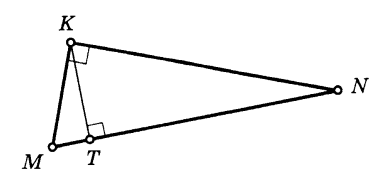
\includegraphics[align=t, width=\linewidth]{../../../../exercises/lists/pics/G81M9L5-10}
			
		\end{minipage}
		\item В треугольнике \( ABC \) на его медиане \( BM \) отмечена точка \( K \) так, что \( BK:KM=4:1 \). Прямая \( AK \) пересекает сторону \( BC \) в точке \( P \). Найдите отношение площади треугольника \( BKP \) к площади треугольника \( ABC \).
		\item 
		\begin{minipage}[t]{\bodywidth}
			На рисунке треугольник \( MOP \) --- равнобедренный, \( OP \) --- его основание, \( MK \) и \( OH \) --- высоты. Докажите, что треугольники \( MOK \) и \( MCH \) подобны и найдите \( CH \), если \( MH=6 \), \( PH=4 \), \( OP=12 \).
		\end{minipage}
		\hspace{0.02\linewidth}
		\begin{minipage}[t]{\picwidth}
			% TODO: \usepackage{graphicx} required
			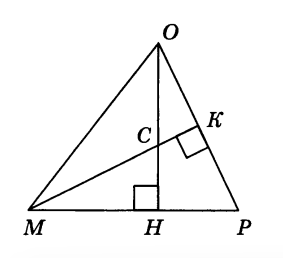
\includegraphics[align=t, width=\linewidth]{../../../../exercises/lists/pics/G81M9L5-1}
		\end{minipage}
		
	\end{listofex}
\end{class}
%END_FOLD

%BEGIN_FOLD % ====>>_____ Занятие 6  _____<<====
\begin{class}[number=6]
	\begin{listofex}
		\item Средние линии треугольника относятся как \( 2 : 3 : 4 \), а периметр треугольника равен \( 45 \) см. Найдите стороны треугольника.
		\item Стороны треугольника равны \( 5 \) см, \( 3 \) см и \( 7 \) см. Найдите стороны подобного ему треугольника, периметр которого равен \( 105 \) см.
		\item Медианы треугольника АВС пересекаются в точке \( O \). Через точку \( O \) проведена прямая, параллельная стороне \( AC \) и пересекающая стороны \( AB \) и \( BC \) в точках \( E \) и \( F \) соответственно. Найдите \( EF \), если сторона \( AC \) равна \( 15 \) см.
		\item  У подобных треугольников сходственные стороны равны \( 7 \) см и \( 35 \) см. Площадь первого треугольника равна \( 27 \) см\( ^{2} \). Найдите площадь второго треугольника.
		\item  Найдите две стороны треугольника, если их сумма равна \( 91 \) см, а биссектриса, проведённая к третьей стороне, делит эту сторону в отношении \( 5:8 \).
		\item В треугольнике \( ABC \) \( AB = 4  \) см, \( BC = 1 \) см, \( AC = 6 \) см, а в треугольнике \( MNK \) \( MK = 8 \) см, \( MN = 12 \) см, \( KN = 14 \) см. Найдите углы треугольника \( MNK \), если \( \angle A = 80\degree \), \( \angle B = 60\degree \).
		\item Прямая пересекает стороны треугольника \( ABC \) в точках \( M \) и \( K \) соответственно так, что \( MK\parallel AC \), \( BM : AM = 1 : 4 \). Найдите периметр треугольника \( BMK \), если периметр треугольника \( ABC \) равен \( 25 \) см.
		\item В треугольнике  \( ABC \)  точка  \( K \)  принадлежит стороне  \( AB \),  а точка  \( P \) --- стороне  \( AC \). Отрезок  \( KP\parallel BC \).  Найдите периметр треугольника  \( AKP \), если  \( AB=9 \) см,  \( BC=12 \) см,  \( AC=15 \) см  и  \( AK : KB=2:1 \).
		\item Диагонали ромба \( ABCD \) пересекаются в точке \( O \), \( BD = 16 \) см. На стороне \( AB \) взята точка \( K \) так, что \( OK \perp AB \) и \( OK = 4\sqrt{3} \) см. Найдите сторону ромба и вторую диагональ.
		\item Отрезки \( AB \) и \( CD \) пересекаются в точке \( O \) так, что \( \angle ACO = \angle BDO \), \( AO : OB = 2:3 \). Найдите периметр треугольника \( ACO \), если периметр треугольника \( BOD  \) равен \( 21 \) см.
		\item Основание треугольника равно \( 36 \). Прямая, паралельная основанию, делит треугольник на две равновеликие части. Найдите длину отрезка этой прямой, заключенного между сторонами треугольника.
		\item Точка \( M \) лежит на боковой стороне \( AC \) равнобедренного треугольника \( ABC \) с основаним \( BC \), причем \( BM=BC \). Найдите \( MC \), если \( BC=1 \) и \( AB=2 \).
	\end{listofex}
\end{class}
%END_FOLD

%BEGIN_FOLD % ====>>_ Домашняя работа 3 _<<====
\begin{homework}[number=3]
	\begin{listofex}
		\item 
		\begin{minipage}[t]{\bodywidth}
			Даны подобные треугольники. Найдите \( x \) и \( y \).
		\end{minipage}
		\hspace{0.02\linewidth}
		\begin{minipage}[t]{\picwidth}
			% TODO: \usepackage{graphicx} required
			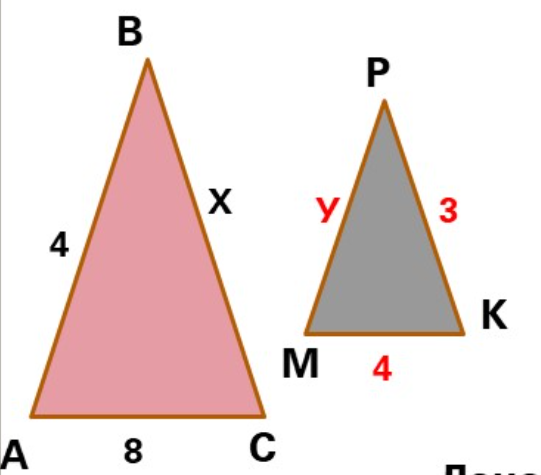
\includegraphics[align=t, width=\linewidth]{../../../../exercises/lists/pics/G81M9H3-1}
		\end{minipage}
		\item Средние линии треугольника относятся как \( 3 : 5 : 6 \), а периметр треугольника равен \( 84 \) см. Найдите стороны треугольника.
		\item \( \triangle ABC \sim \triangle A_1B_1C_1 \), \( AB \) и \( A_1B_1  \) сходственные стороны треугольников, \( AB:A_1B_1=4:3 \), \( AB=8 \) см; \( AC=12 \) см; \( BC=16 \) см. Найдите стороны \( \triangle A_1B_1C_1 \).
		\item \( \triangle MNK \sim \triangle M_1N_1K_1 \) , \( MN=10 \) см, \( MK=12 \) см, \( NK=13 \) см. Периметр \( \triangle M_1N_1K_1 \) равен \( 140 \) см\( ^{2} \). Найдите стороны \( \triangle M_1N_1K_1 \). Найдите площадь \( \triangle M_1N_1K_1 \), если известно, что площадь \( \triangle MNK \) равна \( 32,5 \) см\( ^{2} \).
		\item Периметры подобных треугольников относятся \( 2:3 \), сумма их площадей равна \( 260  \) см\( ^{2} \). Найдите площадь каждого треугольника.
	\end{listofex}
\end{homework}
%END_FOLD

%BEGIN_FOLD % ====>>_____ Занятие 7 _____<<====
\begin{class}[number=7]
	\title{Подготовка к проверочной}
	\begin{listofex}
		\item Занятие 7
	\end{listofex}
\end{class}
%END_FOLD

%BEGIN_FOLD % ====>>_____ Занятие 8 _____<<====
\begin{class}[number=8]
	\begin{listofex}
		\item Занятие 8
	\end{listofex}
\end{class}
%END_FOLD

%BEGIN_FOLD % ====>>_____ Консультация_____<<====
\begin{consultation}[number=7]
	\begin{listofex}
		\item Консультация
	\end{listofex}
\end{consultation}
%END_FOLD
